\documentclass{../mcsslides}

\slidetitle[Часть вторая: архитектурные вопросы]{Лекция 13: Проектирование распределённых приложений}{24.11.2022}

\begin{document}

    \begin{frame}[plain]
        \titlepage
    \end{frame}

    \section{Архитектурные стили распределённых систем}

    % Источник: https://github.com/MicrosoftDocs/architecture-center/tree/main/docs/guide/architecture-styles

    \begin{frame}
        \frametitle{Big Compute}
        \begin{center}
            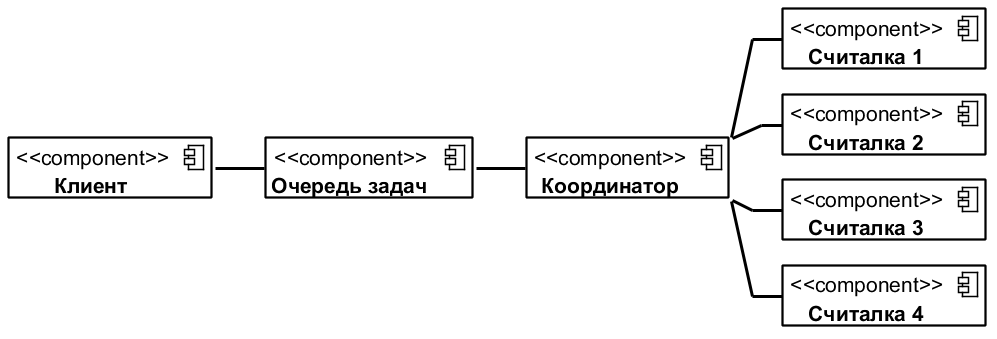
\includegraphics[width=0.8\textwidth]{bigCompute.png}
        \end{center}
        \begin{itemize}
            \item Для сверхсложных задач, предполагающих тысячи вычислительных узлов
            \item Требует <<embarrassingly parallel>> задачу
            \item Предполагает использование весьма продвинутых (и дорогих) облачных ресурсов
        \end{itemize}
    \end{frame}

    \begin{frame}
        \frametitle{Big Data}
        \begin{center}
            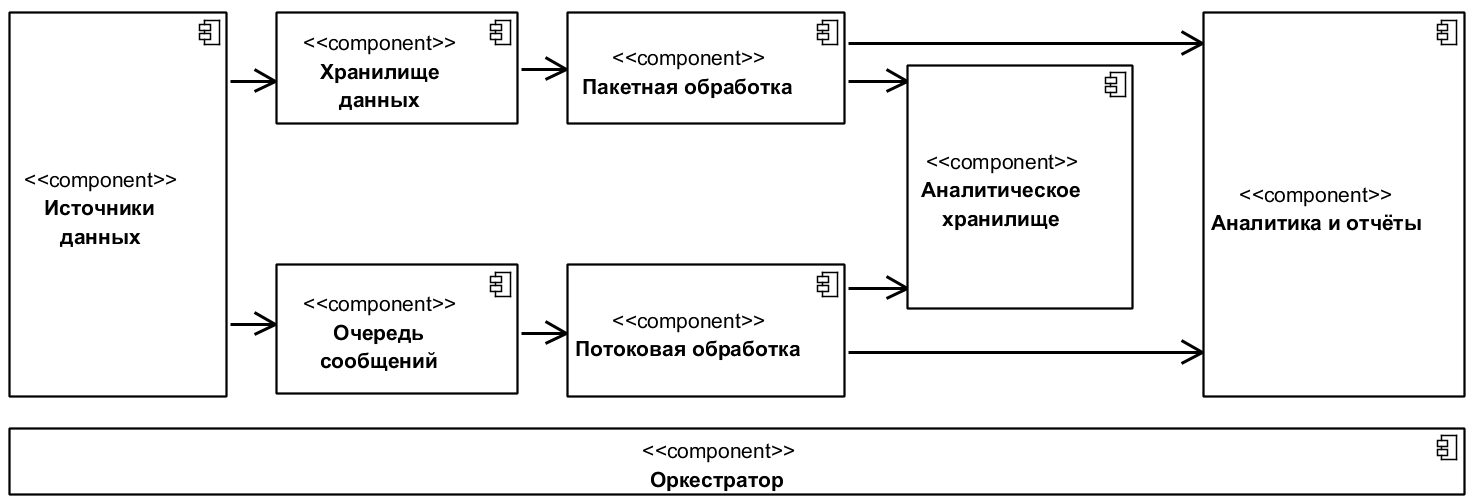
\includegraphics[width=0.9\textwidth]{bigData.png}
        \end{center}
        \begin{itemize}
            \item Для аналитики над большими данными
            \begin{itemize}
                \item Либо данных много и их можно обрабатывать неторопливо
                \item Либо данных много и их надо обрабатывать в реальном времени
            \end{itemize}
            \item Данные не лезут в обычную СУБД
        \end{itemize}
    \end{frame}

    \begin{frame}
        \frametitle{Big Data, хорошие практики}
        \begin{itemize}
            \item Распределённые хранение и обработка
            \begin{itemize}
                \item Например, Apache Hadoop, Apache Spark
            \end{itemize}
            \item Schema-on-read
            \begin{itemize}
                \item Data lake --- распределённое хранилище слабоструктурированных данных
            \end{itemize}
            \item Обработка на месте (TEL вместо ETL)
            \item Разделение данных по интервалам обработки
            \item Раннее удаление приватных данных
        \end{itemize}
    \end{frame}

    \begin{frame}
        \frametitle{Пример: IoT}
        \begin{center}
            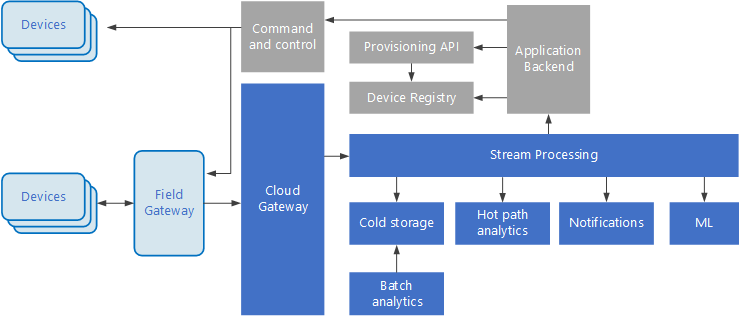
\includegraphics[width=0.9\textwidth]{iot.png}
            \attribution{https://github.com/MicrosoftDocs/architecture-center/blob/main/docs/guide/architecture-styles/big-data.md}
        \end{center}
    \end{frame}

    \begin{frame}
        \frametitle{Событийно-ориентированная архитектура}
        \begin{center}
            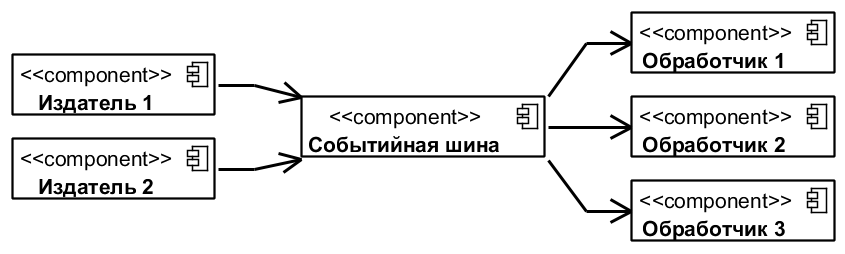
\includegraphics[width=0.7\textwidth]{eventDrivenArchitecture.png}
        \end{center}
        \begin{itemize}
            \item Для обработки событий в реальном времени
            \item Бывает двух видов:
            \begin{itemize}
                \item Издатель/подписчик (например, RabbitMQ)
                \item Event Sourcing (например, Apache Kafka)
            \end{itemize}
        \end{itemize}
    \end{frame}

    \begin{frame}
        \frametitle{Web-queue-worker}
        \begin{center}
            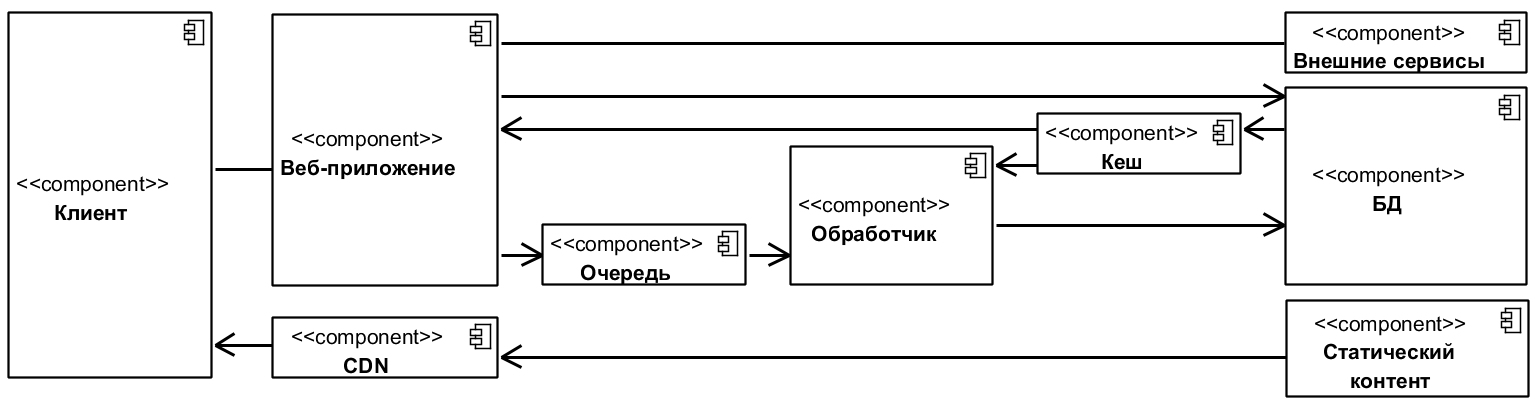
\includegraphics[width=0.9\textwidth]{webQueueWorker.png}
        \end{center}
        \begin{itemize}
            \item Для вычислительно сложных задач в несложной предметной области
            \item Позволяет эффективно использовать готовые сервисы
            \item Независимое масштабирование фронтенда и обработчика
            \item Может превратиться в Big Ball of Mud
        \end{itemize}
    \end{frame}

    \begin{frame}
        \frametitle{N-звенная архитектура}
        \begin{center}
            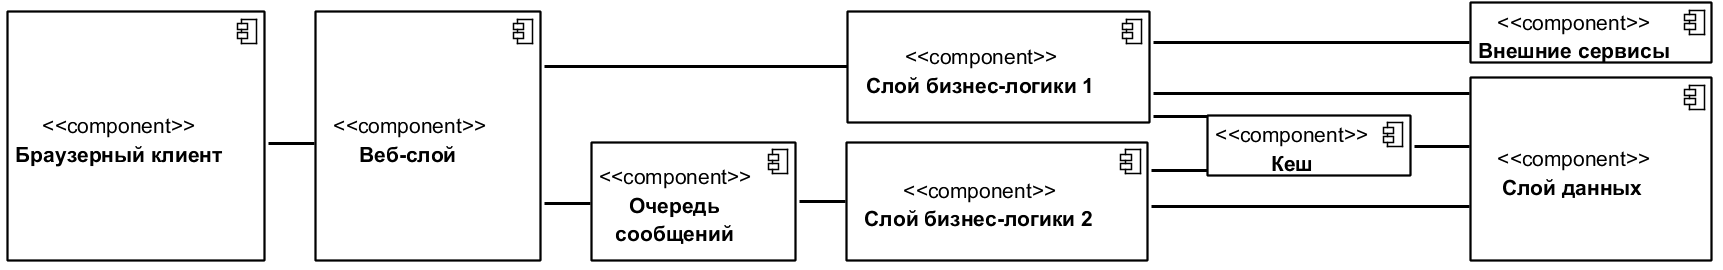
\includegraphics[width=0.9\textwidth]{nTierArchitecture.png}
        \end{center}
        \begin{itemize}
            \item Для быстрого переноса монолита в облако
            \item Для простых веб-приложений
            \item Проблемы с масштабированием и сопровождаемостью
        \end{itemize}
    \end{frame}

    \begin{frame}
        \frametitle{Пример: N-звенное приложение на Azure}
        \begin{center}
            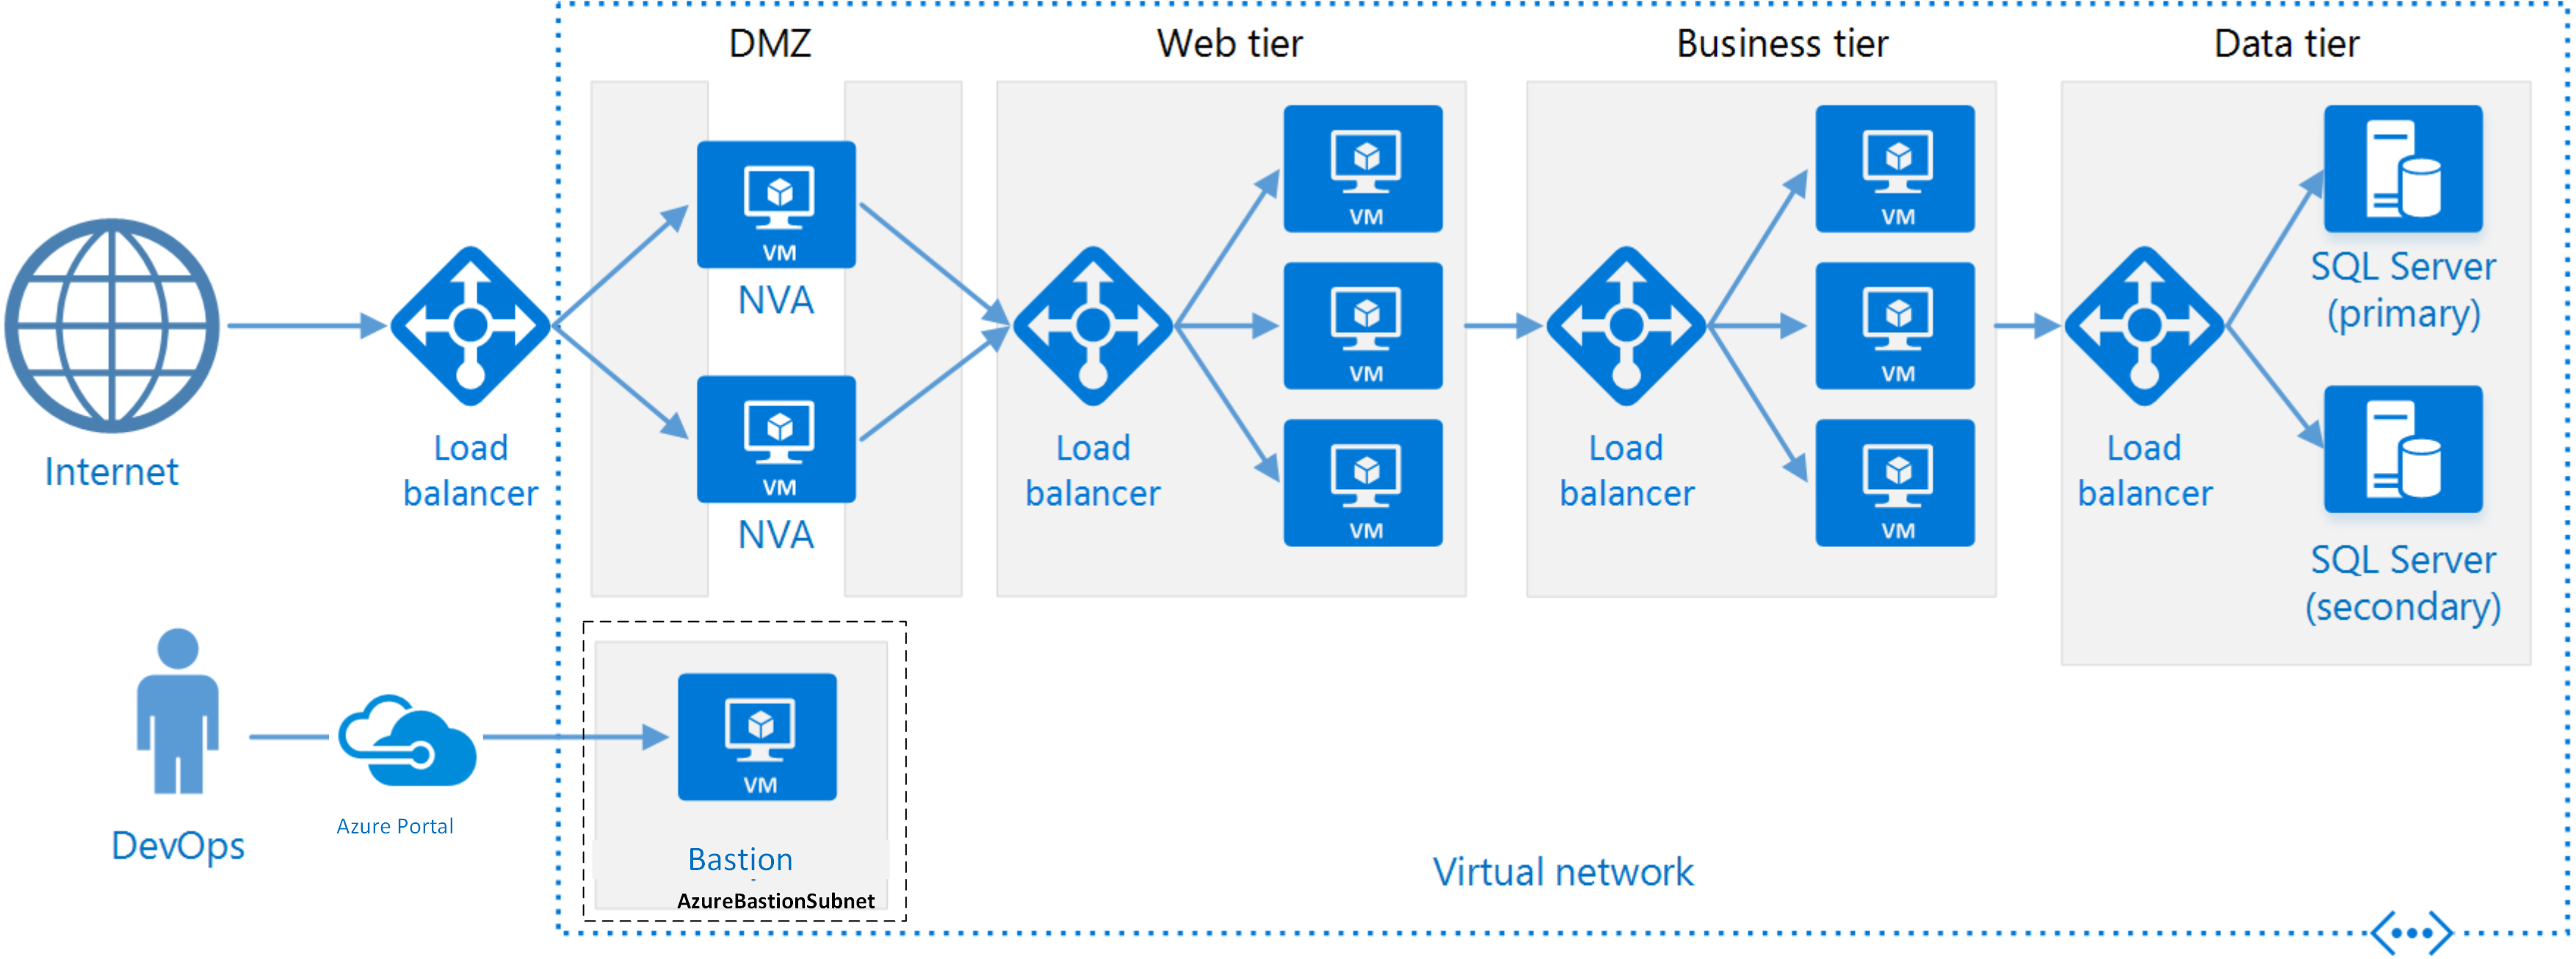
\includegraphics[width=\textwidth]{n-tier-physical-bastion.png}
            \attribution{https://github.com/MicrosoftDocs/architecture-center/blob/main/docs/guide/architecture-styles/n-tier.md}
        \end{center}
    \end{frame}

    \begin{frame}
        \frametitle{Микросервисная архитектура}
        \begin{center}
            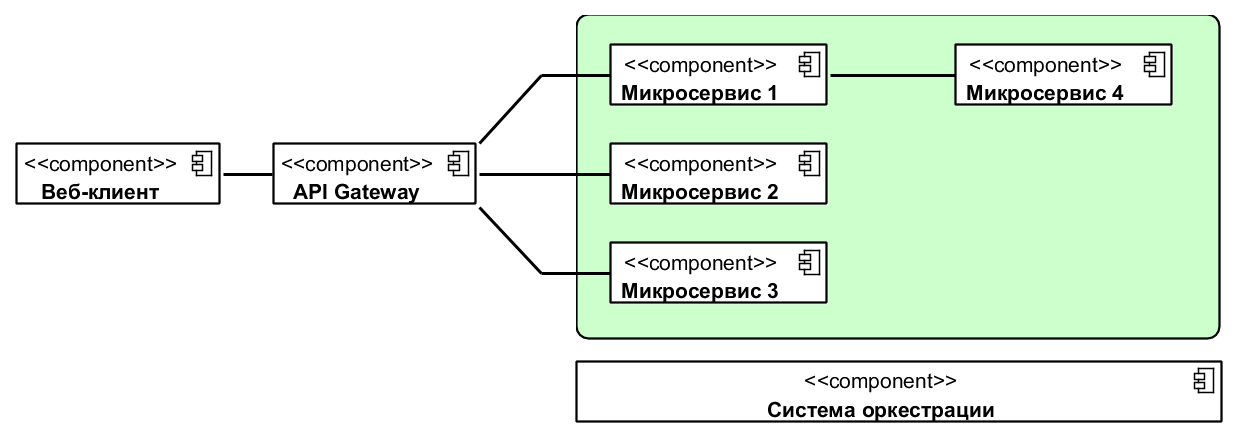
\includegraphics[width=0.85\textwidth]{microservices.png}
        \end{center}
        \begin{itemize}
            \item Для приложений со сложной предметной областью
            \item Альтернатива монолиту, со своими достоинствами и недостатками
            \item Микросервис пишется одним человеком за две недели
            \begin{itemize}
                \item На самом деле, пишется и поддерживается небольшой командой
            \end{itemize}
            \item Микросервис --- ограниченный контекст в смысле DDD
        \end{itemize}
    \end{frame}

    \begin{frame}
        \frametitle{Особенности}
        \begin{itemize}
            \item Каждый микросервис --- отдельное приложение
            \begin{itemize}
                \item Независимость языков и технологий
                \item Имеет своё хранилище данных, не имеет права шарить данные
                \begin{itemize}
                    \item В каком-то смысле, объект из ООП
                    \item Каждому сервису наиболее подходящая СУБД
                \end{itemize}
            \end{itemize}
            \item Мелкозернистая масштабируемость
            \item Независимое развёртывание
            \item Изоляция ошибок
            \item Маленькая и простая кодовая база
        \end{itemize}
    \end{frame}

    \begin{frame}
        \frametitle{Проблемы}
        \begin{itemize}
            \item Сложность перекладывается с реализации на оркестрацию
            \begin{itemize}
                \item Неочевидно, неразвитые инструменты
                \item В целом сложнее, чем рассмотренные выше стили
                \item Сложное управление и мониторинг, требуется развитая культура DevOps
                \item Сложная в плане управления зависимостями разработка
            \end{itemize}
            \item Технологический зоопарк
            \item Нагрузка на сеть
            \item Сложно поддерживать целостность данных
            \begin{itemize}
                \item Eventual Consistency
            \end{itemize}
        \end{itemize}
    \end{frame}

    \section{REST}
    
    \begin{frame}
        \frametitle{Дизайн REST-интерфейса}
        \begin{itemize}
            \item API строится вокруг ресурсов, не действий
            \begin{itemize}
                \item \url{http://api.example.com/customers/} --- хорошо
                \item \url{http://api.example.com/get_customer/} --- плохо
            \end{itemize}
            \item Отношения между сущностями: \url{http://api.example.com/customers/5/orders}
            \begin{itemize}
                \item Максимум одно отношение --- надо будет, сделают ещё запросы
            \end{itemize}
            \item API --- модель предметной области, не данных
            \item Семантика HTTP
            \begin{itemize}
                \item Заголовки Content-Type, Accept
                \item Коды возврата (200, 204, 404, 400, 409)
            \end{itemize}
            \item Механизмы фильтрации и <<пагинации>>
            \item Поддержка Partial Content
            \item Hypertext as the Engine of Application State (HATEOAS)
            \item Версионирование --- не ломать обратную совместимость
        \end{itemize}
    \end{frame}

    \section{Общие принципы дизайна}

    \begin{frame}
        \frametitle{Общие принципы дизайна распределённых приложений}
        \framesubtitle{Самовосстановление}
        \begin{itemize}
            \item Повтор при временном отказе
            \item API для самодиагностики
            \item Разделение на изолированные группы ресурсов
            \item Буферизация запросов
            \item Автоматическое переключение на резервный экземпляр, ручное обратно
            \item Промежуточное сохранение
            \item Плавная потеря работоспособности (graceful degradation)
            \item Тестирование отказов, Chaos engineering
        \end{itemize}
    \end{frame}

    \begin{frame}
        \frametitle{Circuit Breaker, поведение}
        \begin{center}
            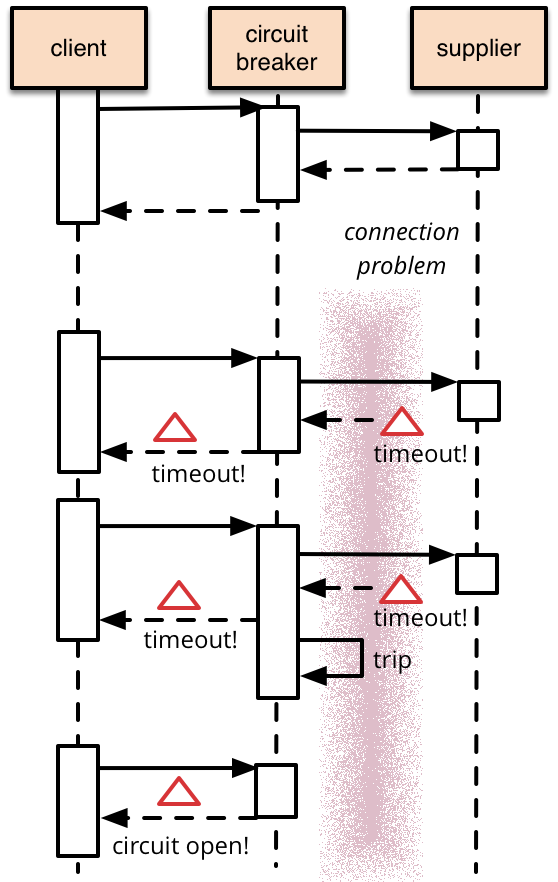
\includegraphics[height=0.7\textheight]{circuitBreakerSequence.png}
            \attribution{\url{https://martinfowler.com/bliki/CircuitBreaker.html}}
        \end{center}
    \end{frame}

    \begin{frame}
        \frametitle{Circuit Breaker, состояния}
        \begin{center}
            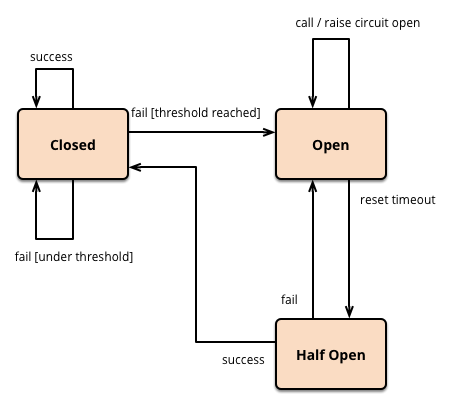
\includegraphics[width=0.5\textwidth]{circuitBreakerStates.png}
            \attribution{\url{https://martinfowler.com/bliki/CircuitBreaker.html}}
        \end{center}
    \end{frame}

    \begin{frame}
        \frametitle{Избыточность}
        \begin{columns}
            \begin{column}{0.5\textwidth}
                \begin{itemize}
                    \item Бизнес-требования к надёжности
                    \begin{itemize}
                        \item Recovery Time Objective, Recovery Point Objective, Maximum Tolerable Outage
                    \end{itemize}
                    \item Балансировщики нагрузки
                    \item Репликация БД
                    \item Разделение по регионам
                    \item Шардирование
                \end{itemize}
            \end{column}
            \begin{column}{0.5\textwidth}
                \begin{center}
                    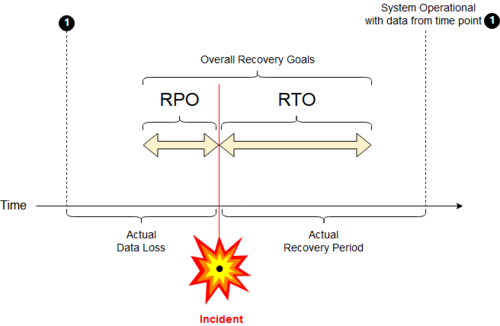
\includegraphics[width=\textwidth]{rpoRtoExample.png}
                    \attribution{\url{https://en.wikipedia.org/wiki/Disaster_recovery}}
                \end{center}
            \end{column}
        \end{columns}
    \end{frame}

    \begin{frame}
        \frametitle{Минимизация координации}
        \begin{itemize}
            \item Доменные события (domain events)
            \item Event Sourcing
            \item Асинхронные, идемпотентные операции
            \item Шардирование
            \item Eventual Consistency, компенсационные транзакции
        \end{itemize}
    \end{frame}

    \begin{frame}
        \frametitle{Command and Query Responsibility Segregation}
        \begin{center}
            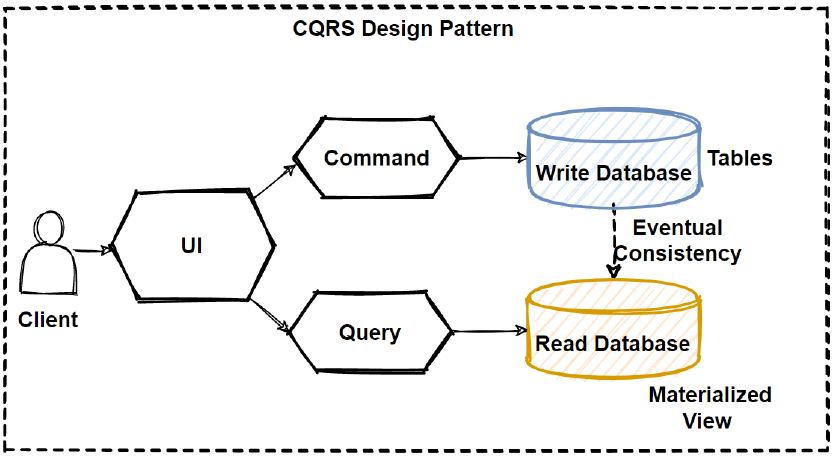
\includegraphics[width=0.8\textwidth]{cqrs.png}
            \attribution{\url{https://medium.com/design-microservices-architecture-with-patterns/cqrs-design-pattern-in-microservices-architectures-5d41e359768c}}
        \end{center}
    \end{frame}

    \begin{frame}
        \frametitle{CAP-теорема}
        В любой распределённой системе можно обеспечить не более двух из трёх свойств:
        \begin{itemize}
            \item Согласованность данных (Consistency) --- во всех вычислительных узлах данные консистентны
            \item Доступность (Availability) --- любой запрос завершается корректно, но без гарантии, что ответы всех узлов одинаковы
            \item Устойчивость к разделению (Partitioning Tolerance) --- потеря связи между узлами не портит ответы
            \begin{itemize}
                \item Этот пункт в распределённых системах должен быть обеспечен всегда, потому что отказы неизбежны. Остаётся выбрать один из двух
            \end{itemize}
        \end{itemize}
    \end{frame}

    \begin{frame}
        \frametitle{ACID vs BASE}
        ACID:
        \begin{itemize}
            \item Atomicity --- транзакция не применится частично
            \item Consistency --- завершённая транзакция не нарушает целостности данных
            \item Isolation --- параллельные транзакции не мешают друг другу
            \item Durability --- если транзакция завершилась, её данные не потеряются
        \end{itemize}
        BASE:
        \begin{itemize}
            \item Basically Available --- отказ узла может привести к некорректному ответу, но только для клиентов, обслуживавшихся узлом
            \item Soft-state --- состояние может меняться само собой, согласованность между узлами не гарантируется
            \item Eventually consistent --- гарантируется целостность только в некоторый момент в будущем
        \end{itemize}
    \end{frame}

    \begin{frame}
        \frametitle{Проектирование для обслуживания}
        \begin{itemize}
            \item Делать всё наблюдаемым
            \begin{itemize}
                \item Трассировка, в т.ч. распределённая
                \item Логирование 
            \end{itemize}
            \item Мониторинг, метрики
            \item Стандартизация форматов логов и метрик
            \item Автоматизация задач обслуживания
            \item Конфигурация --- это код
        \end{itemize}
    \end{frame}

\end{document}
